\chapter{Technical Background}
\section{Introduction}
Satellite geodesy can be considered a multi-parameter estimation problem involving range (distance) or range rate \cite[]{seeber2003chpt2}.  The fundamental equation of satellite geodesy can be expressed as (Figure \ref{fig:chpt2_fig1}).  
\begin{equation} \label{eq:chpt2_eq1}
\begin{aligned}
\textbf{r}_{j}(t)=\textbf{r}_{i}(t)+\boldsymbol{\Delta r}_{ij}(t)
\end{aligned}
\end{equation}
where $\textbf{r}_{j}(t)$ is the satellite position at time $t$, $\textbf{r}_{i}(t)$ is the receiver position at time $t$, and $\boldsymbol{\Delta r}_{ij}(t)$ is the time-varying range between receiver and satellite.  Range is both the observable (sometimes called pseudorange since it is biased by a number of error sources) and a parameter to be estimated.  For Global Positioning System (GPS), receiver position is determined using satellite position and rang estimates.  For Interferometric Synthetic Aperture Radar (InSAR), range change (surface displacement) between two time periods is determined using two or more satellite passes.  For the Gravity Recovery and Climate Experiment (GRACE), rang and range rate between two GPS satellites is observed and used to compute changes in the Earth’s gravity field.  All three techniques rely on precise ranging measurements using the microwave portion of the electromagnetic spectrum, with wavelengths between 0.1 cm and 100 cm and are affected by some common error sources. 

It is useful to distinguish two types of range measurements, one based on signal propagation time and knowledge of the speed of light (sometimes called pseudorange) and carrier phase.  Due to the satellite-receive motion (satellite moves towards or away from receiver during a transmission cycle), carrier phase is sometimes considered equivalent to range rate, also known as accumulated Doppler range.  
Carrier phase is more precise, but suffers from phase ambiguity, which must be solved with additional information.  In GPS, both measurements are used: pseudorange for a “first cut” estimate and then carrier phase for a refined estimate.  In the case of carrier phase ranging, the range between two points can be expressed in terms of the number of whole wavelength and the partial signal wavelength between the transmitter and receiver (\ref{fig:chpt2_fig2}):
\begin{equation} \label{eq:chpt2_eq2}
\begin{aligned}
|\boldsymbol{\Delta r}_{ij}|=N \cdot \lambda +  \frac{\phi}{2\pi} \lambda
\end{aligned}
\end{equation}
where $|\boldsymbol{\Delta r}_{ij}|$ is the range between transmitter and receiver, $\lambda$ is the wavelength of the carrier signal, $N$ is the integer number of signal wavelength, $\phi$ is the phase measurement which is obtained by comparing the original outgoing wave and received incoming wave.  The number of wavelength is unknown or ambiguous.  Resolving the ambiguity of the carrier phase measurement is required for precise ranging.  In GPS, this is known as ambiguity resolution, while in InSAR it is referred to as phase unwrapping.   

Note that carrier phase and pseudorange measurements can be performed in a one-way mode or two-way mode.  One-way ranging is used by GPS and GRACE, while two-way ranging is used for InSAR.   

As shown in Figure\ref{fig:chpt2_fig1}, precise time-dependent satellite position, $r_{j}(t)$, are required in satellite geodesy.  The accuracy of final results of satellite geodesy depends on the accuracy of satellite orbits.  To compute the coordinates of the receiver, it is necessary to know the exact position of each satellite observed.  To a first approximation, knowledge of GPS satellite orbits at the 1 m accuracy level is required to determine the position of a ground receiver at the 1 cm accuracy level.  For InSAR, even tighter constraints on satellite orbits are required.  For GRACE satellites, the satellite orbits are required to relate range and range rate measurement to a global reference frame. 

The microwave signals, when propagating from transmitter to receiver, are subject to atmospheric effect.  For GRACE, this is restricted to ionospheric effects.  For GPS and InSAR, it includes ionospheric effect as well as tropospheric propagation delay. The ionosphere is the upper layer of the Earth’s atmosphere, from about 60 km to 1000 km altitude.  It contains charged particles due to high energy interactions between atmospheric molecules and radiation from the Sun and cosmic rays.  The influence of ionosphere on the propagation of microwave signal is dispersive.  The ionospheric propagation delay depends on the electron density along the signal path as well as the signal frequency.  

The troposphere is the lower layer of the Earth’s atmosphere, from the Earth surface to approximately 15 km altitude.  It contains approximately 75\% of the atmosphere’s total mass and 99\% of its water vapor.   The troposphere is an electrically neutral and its influence on the propagation of microwave signal is non-dispersive.  The tropospheric propagation delay depends on the meteorological status, namely air pressure, partial pressure of water vapor, pressure of dry gas and temperature.  For all three techniques, atmospheric effects have to be determined and corrected in order to obtain high precision results.

\section{Global Positioning System}
The Global Positioning System (GPS) was developed by the U.S Department of Defense (DoD) to provide civilian and military users with worldwide positioning, navigation and timing services.  The position measurements can be used to study the movements of the Earth surface (deformation) associated with different Earth processes.  Here, a brief introduction about the principles of GPS and errors sources of the GPS position measurement is presented.  For detailed studies, the reader is referred to \citet{dixon1991chpt2},\citet{mao1999chpt2} and \citet{hofmann2001chpt2}. 

\subsection{Structure}
The GPS system consists of three segments: the space segment, the control segment, and the user segment.  The space segment consists of the GPS satellites that transmit radio signals to users.  The nominal GPS constellation consists 24 satellites that are equally spaced in 6 orbital planes with 4 satellites in each plane (Figure \ref{fig:chpt2_fig3}).  Orbital planes are 60 degree separated and inclined at about 55 degrees with respect to the equatorial plane.  Each satellite flies in high Earth orbit at an altitude of about 20200 km, circling the Earth twice per day.  This constellation ensures that users can view at least 4 satellites from any point on the Earth at any time. The control segment on the ground consists of a system of facilities that receive signals from the satellites, perform analysis to compute satellite orbital data (ephemerides) and clock corrections, and send ephemerides back to each satellite for re-broadcast to users.  The user segment consists of the GPS receivers that receive the signals from the GPS satellite and convert them into three-dimensional position, time and other parameters.  

\subsection{GPS signal}
Each GPS satellite transmits microwave signals on two carrier frequencies: L1 (1575.42 MHz) and L2 (1227.60 MHz).  Two pseudorandom noise (PRN) codes and broadcast message (data signal) are modulated onto the carrier frequencies.  The PRN codes are a sequence of binary values which look like random electrical noise to users without code knowledge.  Maximum autocorrelation can be achieved when two code sequences coincide exactly, allowing determination of signal travel time.   Two types of PRN codes are used: the Precision (P) code and the Coarse/Acquisition (C/A) code.  The main features of carrier, code and data signals are shown in Table \ref{tab:chpt2_table1}. 

The C/A code is modulated onto the L1 carrier. The P code is modulated onto the L1 and L2 carriers.  The P-code is encrypted into Y-code in the Anti-Spoofing (AS) mode, which denies access by unauthorized users (Figure \ref{fig:chpt2_fig4}).  Note that as a major focus of the GPS modernization program, a new military (M) signal and three new civil (L1C, L2C, L5) have been added to the L1 and L2 carriers. 

\subsection{GPS basic observations}
To determine three-dimensional position of a user, the GPS receiver should compute the range to at least four satellites, combined with knowledge of satellites positions at the time of signal transmission.  However, due to lack of synchronicity between satellite clock and receiver clock, plus other factors, the GPS receiver can only provide pseudorange measurements rather than the true geometric range.  GPS receivers provide two types of pseudorange observations: code pseudorange and carrier phase pseudorange.  The code pseudorange is obtained by multiplying the speed of light by the travel time, where the travel time is determined by correlating the received code (C/A or P(Y)) from the satellite with the replicas generated by the receiver.  The carrier phase pseudorange is obtained by multiplying the wavelength by difference between carrier phase from the satellite and the carrier phase generated by the receiver.  Carrier phase pseudorange is about two orders of magnitude more precise than the code pseudorange, but the carrier phase observation is ambiguous by an integer number of cycles \cite[]{remondi1985chpt2}.  In order to achieve millimeter-precision, the ambiguity problem must be fixed.  Carrier phase ambiguity resolution has been studied by \citet{lichten1987chpt2} and \citet{blewitt1989chpt2,blewitt2008chpt2}.  

\subsection{GPS error sources}
There are many sources of error contaminating the GPS position measurements. Major GPS error sources are briefly discussed below.  For a detailed description, the reader is referred to \citet{hofmann2001chpt2}.  

(i) Satellite clock and orbit errors
 
GPS satellite clock time should be synchronous with GPS time (the time scale used by the GPS system).  Errors in the satellite clock estimate have a major impact on the computed code pseudorange.  Similarly, errors in the satellite orbit estimate can corrupt the ground position estimate.  In this dissertation, I use the precise final orbits and adjusted clock products provided by the Jet Propulsion Laboratory to mitigate satellite clock and orbit errors.  Another source of precise satellite orbits and adjusted clock products is the International GNSS Service (IGS). 

(ii) Atmospheric effects 

The GPS signals are refracted by ionosphere and troposphere, causing ray benging and changing the propagation time.  The first-order effects of the ionosphere can be corrected using the dual-frequency approach and a linear combination of carrier phase measurements.  The remaining high-order ionospheric effects are less than 1 mm \cite[]{hernandez2007chpt2,petrie2010chpt2}.  The tropospheric effects can be reduced by using an elevation mask to avoid receiving signals from satellites lower than a certain elevation.  The tropospheric delay must be modeled.  The tropospheric model consists of mean tropospheric parameters or measurements data (temperature, air pressure, water vapor) and a mapping function \cite[]{niell1996chpt2,boehm2006chpt2,boehm2007chpt2}.

(iii) Multipath effects 

The following section is summarized from the work of \citet{larson2007chpt2}.  The receiver antenna gets a direct signal through a straight-line path, plus reflected signals through multiple paths.  The path length of the reflected signal is longer than the direct signal, causing errors to both code and carrier-phase observations, which then propagate into position solutions.  Multipath effects on code observation are much larger than on the carrier-phase observation.  Two types of multipath exist: diffuse multipath and specular multipath.  Diffuse multipath occurs when the GPS signal reaches a rough surface and the reflected signal is scattered in multiple directions.  Diffuse multipath causes unbiased and time-uncorrelated errors which can be easily to remove through real-time signal filtering in the receiver.  Specular multipath occurs when the GPS signal reaches a smooth surface and then is reflected into a single direction.   In contrast to errors caused by diffuse multipath, errors caused by specular multipath are systematic and time-correlated which cannot be removed by traditional filtering methods.   To date there is no widely used model for multipath effect correction since the multipath-generating environment is dynamic and it is unique for each GPS site.  Various approaches have been developed to for multipath effect reduction and correction.  For example, one can estimate the multipath corrections from SNR data \cite[e.g.,][]{axelrad1996chpt2} or mitigate the multipath errors using the sidereal filtering technique, replying upon the repeating orbital characteristics of the GPS satellites \cite[e.g.,][]{genrich1992chpt2,choi2004chpt2}.  The aspect repeat time adjustment (ARTA) technique has also been suggested to maximize the effectiveness of techniques relying upon the geometric repeatability of GPS satellite orbits \cite[]{larson2007chpt2}.  In our processing routine, we estimate observations every 24 hours to minimize the multipath error \cite[]{sella2002chpt2}.  

(iv) Antenna phase center offset and variation 

The electrical antenna phase center (APC) is the point in space where radio signal is received.  However, the position of the APC varies depending on the intensity and direction of the incoming signal.  Thus, antenna phase center variation (PCV) is defined as the difference between the APC of each measurement and the mean position of the electrical antenna phase center (MPC).   The antenna phase center offset (PCO) is defined as the difference between MPC and antenna reference point (ARP) given by the manufacture.  \citet{steigenberger2006chpt2} reprocessed years of GPS data and estimated the antenna phase center offsets for a variety of GPS receivers.  An absolute phase center correction model estimated by \citet{schmid2007chpt2} can be use to calibrate both GPS satellite and receiver antennas.  

Note that only the major error sources are discussed here.  Other factors such as receiver clock error, monument movement and software accuracy (e.g., mis-modeling of key physical processes) also cause errors in the GPS position measurement.  Last but not least, deformations due to ocean tidal and atmospheric loading need to be modeled and removed so that the geophysical process of interest (e.g., ice mass loss) can be separated from other geophysical processes.  The specific models used are describe below.    

In this dissertation, GPS analysis is conducted with the Precise Point Positioning software developed by JPL GIPSY/OASIS \cite[]{zumberge1997chpt2}.  JPL's precise orbits and clock products are used to generate daily point position solutions.  The dual-frequency approach and a linear combination of carrier phase measurements are used for correcting the first-order effects of the ionospheric effect.  Tropospheric effects are modeled using the Global Mapping Function \cite[]{boehm2006chpt2}.  The elevation cut-off angle is chosen to 7 \textordmasculine in order to better constrain tropospheric effects meanwhile to minimize multipath errors.  The ocean loading effects are corrected using the FES2004 model \cite[]{lyard2006chpt2}.  The non-tidal atmospheric loading effects are corrected using a global 2.5 $\times$ 2.5 degree displacement field computed from a model provided by the National Center for Environmental Protection \cite[]{petrov2004chpt2}.  The Ambizap algorithm \cite[]{blewitt2008chpt2} is adopted to solve integer ambiguities for each station.  The non-fiducial daily solutions are then aligned to the IGS05 reference frame \cite[]{altamimi2007chpt2} using JPL's X-files, a 7-parameter transformation.  

\section{Interferometric Synthetic Aperture Radar}
Interferometric Synthetic Aperture Rader (InSAR) is a radar technique for mapping the Earth topography and/or Earth surface deformation using an inteferogram formed by two Synthetic Aperture Radar (SAR) images.  Using InSAR to study Earth surface deformation is briefly summarized here. The reader is referred to \citet{curlander1991chpt2}, \citet{massonnet1998chpt2}, \citet{rosen2000chpt2} and \citet{hanssen2001chpt2} for more detailed reviews.  

\subsection{Basic concept}
A satellite borne Synthetic Aperture Radar (SAR) transmits a pulse of microwave signals to illuminate a target area on the Earth and then receives the returned signal scattered by the Earth’s surface.  The returned signal contains two kinds of information: amplitude and phase, which are recorded in a two-dimensional radar image.  The amplitude is a measure of target reflectivity, which reflects the physical properties of ground target.  The phase corresponds to the fractional part of the round trip range between satellite antenna and ground target.  Current satellite borne SARs typically work in three microwave bands: X-band (wavelength of $\sim$ 3 cm), C-band (wavelength of $\sim$ 6 cm) and L-band (wavelength of $\sim$ 24 cm).  With a high bandwidth microwave signal and the synthetic aperture technique (transmit and receive signals using a radar antenna installed on a moving platform), satellite borne SAR image can achieve high spatial resolution. 

InSAR uses two SAR images to produce an interferogram which contains the phase difference (also called interferometric phase, $\phi$) between every pair of corresponding pixels in two SAR images.  The range change ($R_{2}-R_{1}$) between two image acquisitions is then measured in terms of the interferometric phase ($phi$): 
\begin{equation} \label{eq:chpt2_eq3}
\begin{aligned}
\phi=\frac{4 \pi}{\lambda}(R_{2}-R_{1})
\end{aligned}
\end{equation}
where $lambda$ is the carrier wavelength, $R_{1,2}$ is the range from satellite antenna A$_{1,2}$ to the ground target (Figure \ref{fig:chpt2_fig5}).  As with GPS, the phase of SAR image is ambiguous because it is only the fractional part of the change in phase.  Therefore, the interferometric phase needs to be unwrapped.  Phase unwrapping is a critical step for using InSAR to monitor topography or surface deformation and various approaches have been developed to solve the problem \cite[e.g.,][]{zebker1998chpt2}.  

\subsection{Monitoring surface deformation}
If the two SAR images are acquired from slightly different viewing points at different times, any movement of the ground target with a component projected onto the line of sight (LOS) of the radar beam gives the deformation phase: 
\begin{equation} \label{eq:chpt2_eq4}
\begin{aligned}
\phi_{def}=\frac{4 \pi}{\lambda}(\delta R)
\end{aligned}
\end{equation}
where $\phi_{def}$ is the interferometric phase caused by surface deformation; $\lambda$ is the carrier wavelength; $\delta R$ is the range change, which is the surface displacement projected onto the LOS of the radar beam.  Theoretically, if $\phi_{def}$ is known, the surface displacement can be determined at millimeter-precision.  However, besides deformation phase, other phase terms also contribute to the interferometric phase measurement ($\phi$):
\begin{equation} \label{eq:chpt2_eq5}
\begin{aligned}
\phi= \phi_{def} + \phi_{topo} + \phi_{atm} + \phi_{orb}
\end{aligned}
\end{equation}
where $\phi_{topo}$,$\phi_{atm}$ and $\phi_{orb}$ are the phase due to range changes associated with topography, atmospheric effects and orbit errors.  In order to monitor surface deformation, $\phi_{topo}$,$\phi_{atm}$ and $\phi_{orb}$ should be removed from $\phi$.

(i) Topography
 
In most cases, two SAR images are taken from slightly different viewing points (A$_{1,2}$) so that the interferometric phase contains the topographic component (Figure \ref{fig:chpt2_fig5}).  A Digital Elevation Model (DEM) is used to represent the topography. Thus, if an accurate DEM is available, the topographic phase can be estimated and then subtracted from the interferometric phase.  Note that errors in the DEM cause tropospheric phase residuals in the deformation phase.  In place of a DEM, the differential InSAR technique can be used to separate topographic phase from deformation phase.  Two or more interferograms with different baselines are differenced to produce differential interferograms.  In practice, along with topographic phase the reference phase induced by acquisition geometry is estimated and subtracted from the interferometric phase. 

(ii) Atmospheric effects 

As with GPS, it is important to consider atmospheric effects on monitoring surface deformation using InSAR \cite[]{goldstein1995chpt2,zebker1997chpt2}. The state of atmosphere changes if the two images are acquired at different times.  Atmospheric heterogeneity leads to differences in atmospheric delay and hence the phase difference. Temporal and spatial variations of atmospheric pressure, temperature and water vapor all leads to errors in deformation.  Particularly large errors ($\sim$10 cm) in deformation measurements can result from variations (20\%) of atmospheric water vapor \cite[]{zebker1997chpt2}.  Producing robust estimates of atmospheric delay remains to be one of the challenges in improving the accuracy of surface deformation with the InSAR technique.  A variety of methods have been proposed to reduce the effects of atmospheric delay, including averaging multiple interferograms to cancel out uncorrelated atmospheric delay \cite[e.g.,][]{zebker1997chpt2}, spatial-temporal filtering \cite[e.g.,][]{berardino2002chpt2}, and using complementary data such as GPS data and meteorological models to estimate atmospheric delay \cite[e.g.,][]{williams1998chpt2,foster2006chpt2,jolivet2014chpt2}.

(iii) Orbital errors
Errors in the satellite orbits are a limitation for InSAR in measuring surface deformation accurately.  To remove both tropographic phase and reference phase (together called geometric phase), precise satellite orbits are required to determine the interferometric baseline to millimeter precision.  However, orbits of most remote sensing satellites are much less precise, e.g., 10 cm – 1m \cite[]{yoon2009chpt2,eineder2011chpt2,rudenko2012chpt2}, hence the interferometric baseline cannot be precisely determined directly. Therefore, orbital errors contributes to phase difference in the interterograms.  Several methods have been proposed to reduce the effects of orbital errors.  A simple but widely used method is to estimate a planar phase ramp that fits to interferometric phases \cite[]{massonnet1998chpt2}. 

Besides the factors discussed above, phase noise induced by the radar system (e.g., thermal noise), changes in the scattering behavior of the ground target (e.g., changes in dielectric constant), and data processing (e.g., phase unwrapping) errors also contribute to the interferometric phase, all inducing errors in the InSAR measurements.  

\section{Gravity Recovery and Climate Experiment}
Launched in March 2002, the Grace Recovery and Climate Experiment (GRACE) mission makes detailed measurements of the time varying gravity field of the Earth with a spatial resolution of $\sim$ 300 km \cite[]{tapley2004chpt2,wahr2004chpt2}.    GRACE measures gravity variations that are related to the redistributions of mass in the solid Earth and its fluid envelope.  Currently, many studies focus on mass redistribution processes occurring in the hydrosphere, cryosphere and the ocean, which are within a thin layer at the Earth’s surface.  Here, the principle of GRACE measurement and its application in measuring the Earth’s surface mass change are briefly summarized.  The reader is referred to \citet{wouters2014chpt2} for more a detailed review. 

\subsection{Basic concept}
GRACE consists of two identical satellites at altitude of about 500 km, one following the other in a low, near-circular, near-polar orbit with an inclination of 89 \textordmasculine, $\sim$ 220 km apart along-track (Figure \ref{fig:chpt2_fig6}).  A highly accurate inter-satellite, K-Band microwave range (KBR) system, continuously measures the range between two satellites.  Each satellite transmits carrier phase to the other at dual-frequency (24 and 32 GHz), allowing for ionospheric correction during data processing.  Each satellite receives the carrier phase and compares it with the on-board generated phase in order to obtain the range between two satellites.  Changes in range contains gravitational information: the leading satellite accelerates when passing an area of stronger gravity (anomaly), resulting in range increase between the two satellite; the leading satellite then decelerates when past the anomaly and the trailing satellite accelerates, resulting in a range decrease.  In addition to the KBR system, each satellite is equipped with a GPS receiver, a high precision accelerometer and star cameras.  The GPS receiver provides the position of two GRACE satellites and the time-tags of KBR measurements.  The accelerometer is used to measure the surface force acceleration so that the effects of non-gravitational forces, such as air drag and solar radiation pressure, can be removed from the range-rate measurement.  The star cameras are used to measure the orientation of satellites in space so that the K-Band antennas are pointing towards each other precisely.  

\subsection{Data Products}
The GRACE gravity data products are developed, processed and archived by three centers within a shared Science Data System (SDS): Jet Propulsion Laboratory (JPL), the Center for Space Research at the University of Texas (UTCSR), and the Geoforschungszentrum in Potsdam (GFZ).  The GRACE gravity data product is divided into three levels: Level-0, Level-1, Level-2.  

Level-0 data is the raw data from GRACE satellite.  It is the result of telemetry data reception, collection and documentation by the Raw Data Center (RDC) of the Mission Operation System (MOS) in Germany. Level-0 data product is not available to the public.  

Level-1 data product is divided into two levels: Level-1A and Level-1B.  Level-1A data product is the result of reversible processing applied to the Level 0 data.  The data is calibrated, time-tagged to the respective satellite receiver clock time and reformatted for further processing.  Level-1B data product is the result of extensive and irreversible processing applied to Level-0 and Level-1A data products.  The data is correctly time-tagged and the data sample rate is reduced from 10 Hz to 0.1 Hz.  Level-1B data product includes inter-satellite range, range-rate, range-acceleration, the non-gravitational acceleration for each satellite, etc.  Level-1B data product is available to the public.  

Level-2 data are processed by JPL, GFZ and UTCSR independently and are released to the public through two portals: the Physical Oceanography Distributed Active Archive Center (PO.DAAC) at JPL and the Information System \& Data Center (ISDC) at GFZ.   Level-2 data products include the orbit of the GRACE satellites, monthly and mean estimates of spherical harmonic (Stokes) coefficients (C$_{lm}$, S$_{lm}$) of the Earth gravity field.  Note that the degree ($l$) and order ($m$) of the Stokes coefficients are up to 60 for CSR and 120 for JPL and GFZ.  Most scientific studies based on GRACE measurements utilize Level-2 data products.  The latest version of the gravity field coefficients is Release-05, which is more accurate than the previous versions based on better knowledge of on-board instruments (star cameras, accelerometer and the KBR system) and updated mean gravity field and other background force models (e.g., ocean tide model, pole tide model, etc) for Level-2 processing \cite[]{chambers2012chpt2}.  

\subsection{Measuring the Earth's surface mass change}
How do we use GRACE gravity data to measure the surface mass change?  Here, we consider surface mass change as a thin layer of water on the Earth’s surface with varying thickness.  According to \citet{wahr1998chpt2}, the surface mass density $\Delta \sigma$ [kg m$^{-2}$] can be expressed as:
\begin{equation} \label{eq:chpt2_eq6}
\begin{aligned}
\Delta \sigma(\phi,\lambda) = \frac{a_{e} \rho_{e}}{3} \sum_{l=0}^{\infty} \sum_{m=0}^{l} \frac{2l+1}{1+k_{l}} P_{lm} (cos \phi) [\Delta C_{lm}\cos(m\lambda)+\Delta S_{lm}\sin(m \lambda)]
\end{aligned}
\end{equation}
where $phi$,$lambda$ are the colatitude and longitude of a point above the Earth’s surface, $a_{e}$ is the mean equatorial radius of the Earth, $\rho_{e}$ is the mean density of the Earth, $l$ and $m$ are the degree and order of the spherical harmonic coefficients, $k_{l}$ is the Love number of degree $l$,   is the Legendre Polynomials of degree $l$ and order $m$,   and  are the coefficients for some month of $l$ degree and m order released by GRACE.  Many studies report mass change using changes in height of water by dividing $\Delta \sigma$ [kg m$^{-2}$] by the density of water $rho_{w}$ [kg m$^{-3}$].

Several processing procedures need to be applied to the GRACE gravity field solutions in order to estimate surface mass change correctly.  

(i) Striping effect
Spatially correlated errors in the Stokes coefficients cause the north-south oriented stripes in maps of surface mass change, which is called the striping effect (Figure \ref{fig:chpt2_fig7}a).  Such errors are prominent in the high degree Stokes coefficients.  Several techniques have been developed to reduce the striping effect in the gravity field solution.  One common technique is Gaussian smoothing (Figure \ref{fig:chpt2_fig7}c), which use a bell-shaped Gaussian kernel to ‘blur’ images and remove detail and noise.  The Gaussian kernel is isotropic, meaning that the behavior of the function is the same in any direction.  However, the stripping effect in GRACE data is non-isotropic, orienting in North-South direction.  Therefore, some no-isotropic kernels are developed to reduce the stripping effects \cite[e.g.,][]{chen2006chpt2,kusche2009chpt2}.  \citet{swenson2006chpt2} developed a correlated-error filter which further reduce the noise in GRACE data (Figure \ref{fig:chpt2_fig7}).  

(ii) Leakage effects

The limited spatial resolution of the GRACE gravity field solution and spatial smoothing causes leakage, where signals do not concentrated solely over the region of mass variation but spread out into nearby regions artificially \cite[e.g.,][]{chen2006antarctic}.  Thus, the surface mass variation over a region of interest could be contaminated by signals leaking from nearby regions, or by signals leaking out to nearby regions. It is important to identify and correct leakage effects in order to obtain correct estimates of surface mass change using GRACE gravity data.  Using an averaging function is a simple method to minimize the combined measurement error and leakage error, and the result is then scaled to avoid signal attenuation \cite[]{velicogna2006chpt2}.  The mascon technique is utilized to better localize the mass variation over a relatively small region \cite[]{rowlands2005chpt2}.  The original KBR range rate data and the analytical skills are required to produce the Gravity field solution using the mascon technique, making this technique less doable for most GRACE users.  \citet{schrama2011chpt2} proposed an inversion modeling technique based on a least squares approximation method to estimate the optimized uniform mass variation in each block.  The inversion modeling technique is useful to estimate surface mass changes in high spatial resolution and is easy to use.  

(iii) Glacial Isostatic Adjustment

Glacial isostatic adjustment (GIA) is the ongoing movement of the lands that were depressed by ice sheets during the last glacial period.  The redistribution of lithospheric masses, adjusting from the ice sheet loading state back to the equilibrium state, causes long-term trends in the Earth’s gravity field.  To study the current surface mass changes, it is important to quantify and separate the long-term trend caused by GIA from the current signal of interest.  The GIA model is composed of an ice model and the Earth rheology model.  The ice model describes the loading and unloading history of ice sheets.  The Earth rheology model describes the redistribution of lithospheric masses forced by the surface loading and unloading events.  The present-day crustal uplift data are used to calibrate GIA models.  Although it is possible to model the GIA effect and subtract it from the GRACE data, it is challenging to predict the GIA effect accurately \cite[]{thomas2011chpt2}.  Thus, GIA effect remains one of the error sources of surface mass change using GRACE gravity data.  

\section{References}
\bibliographystyle{apalike}  
\bibliography{chpt2_ref}

\clearpage
\begin{table}[h!]
	\begin{center}
		\caption{GPS satellite signals (bps = bits per second) \cite[]{seeber2003chpt2}}
		\label{tab:chpt2_table1}
		\begin{tabular}{ll}
			\midrule
			Atomic clock fundamental frequency & 10.23 MHz \\
			\midrule
			L1 frequency & 1575.42 MHz\\
			L1 wavelength & 19.0 cm\\
			L2 frequency & 1227.60 MHz\\
			L2 wavelength & 24.4 cm\\
			\midrule
			P-code frequency & 10.23 MHz\\
			P-code wavelength & 29.31 m\\
			P-code period & 266 days\\
			C/A-code frequency & 1.023 MHz\\
			C/A-code wavelength & 293.1 m\\
			C/A-code period & 1 millisecond\\
			\midrule
			data signal frequency & 50 bps\\
		    data signal cycle length & 30 seconds\\			
			\midrule
		\end{tabular}
	\end{center}
\end{table}
 
\clearpage
\begin{figure}
	\centering
	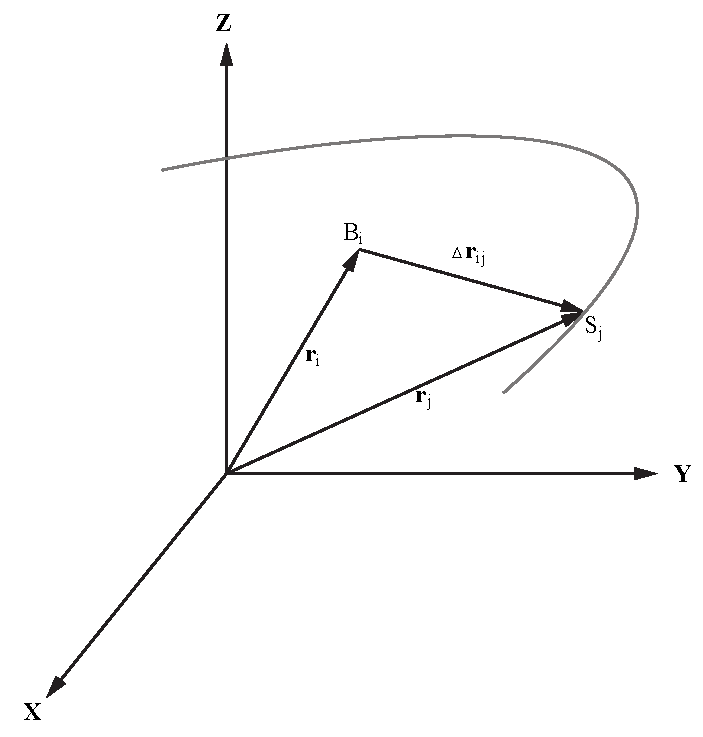
\includegraphics{figs_chpt2/Fig1.pdf}	
	\caption[Basic relations for satellite observations.]{Basic relations for satellite observations (Figure 4.1 in \citet{seeber2003chpt2}). $B$ represents the receiver and $S$ represents the satellite.}
	\label{fig:chpt2_fig1}
\end{figure}

\clearpage
\begin{figure}
	\centering
	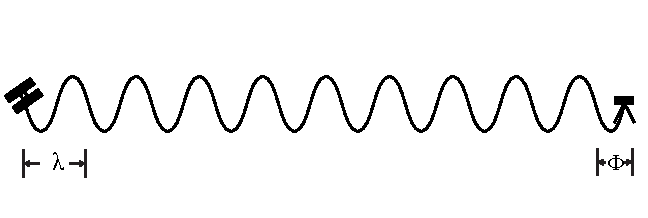
\includegraphics{figs_chpt2/Fig2.pdf}	
	\caption[Carrier phase ranging.]{Carrier phase ranging.}
	\label{fig:chpt2_fig2}
\end{figure}

\clearpage
\begin{figure}
	\centering
	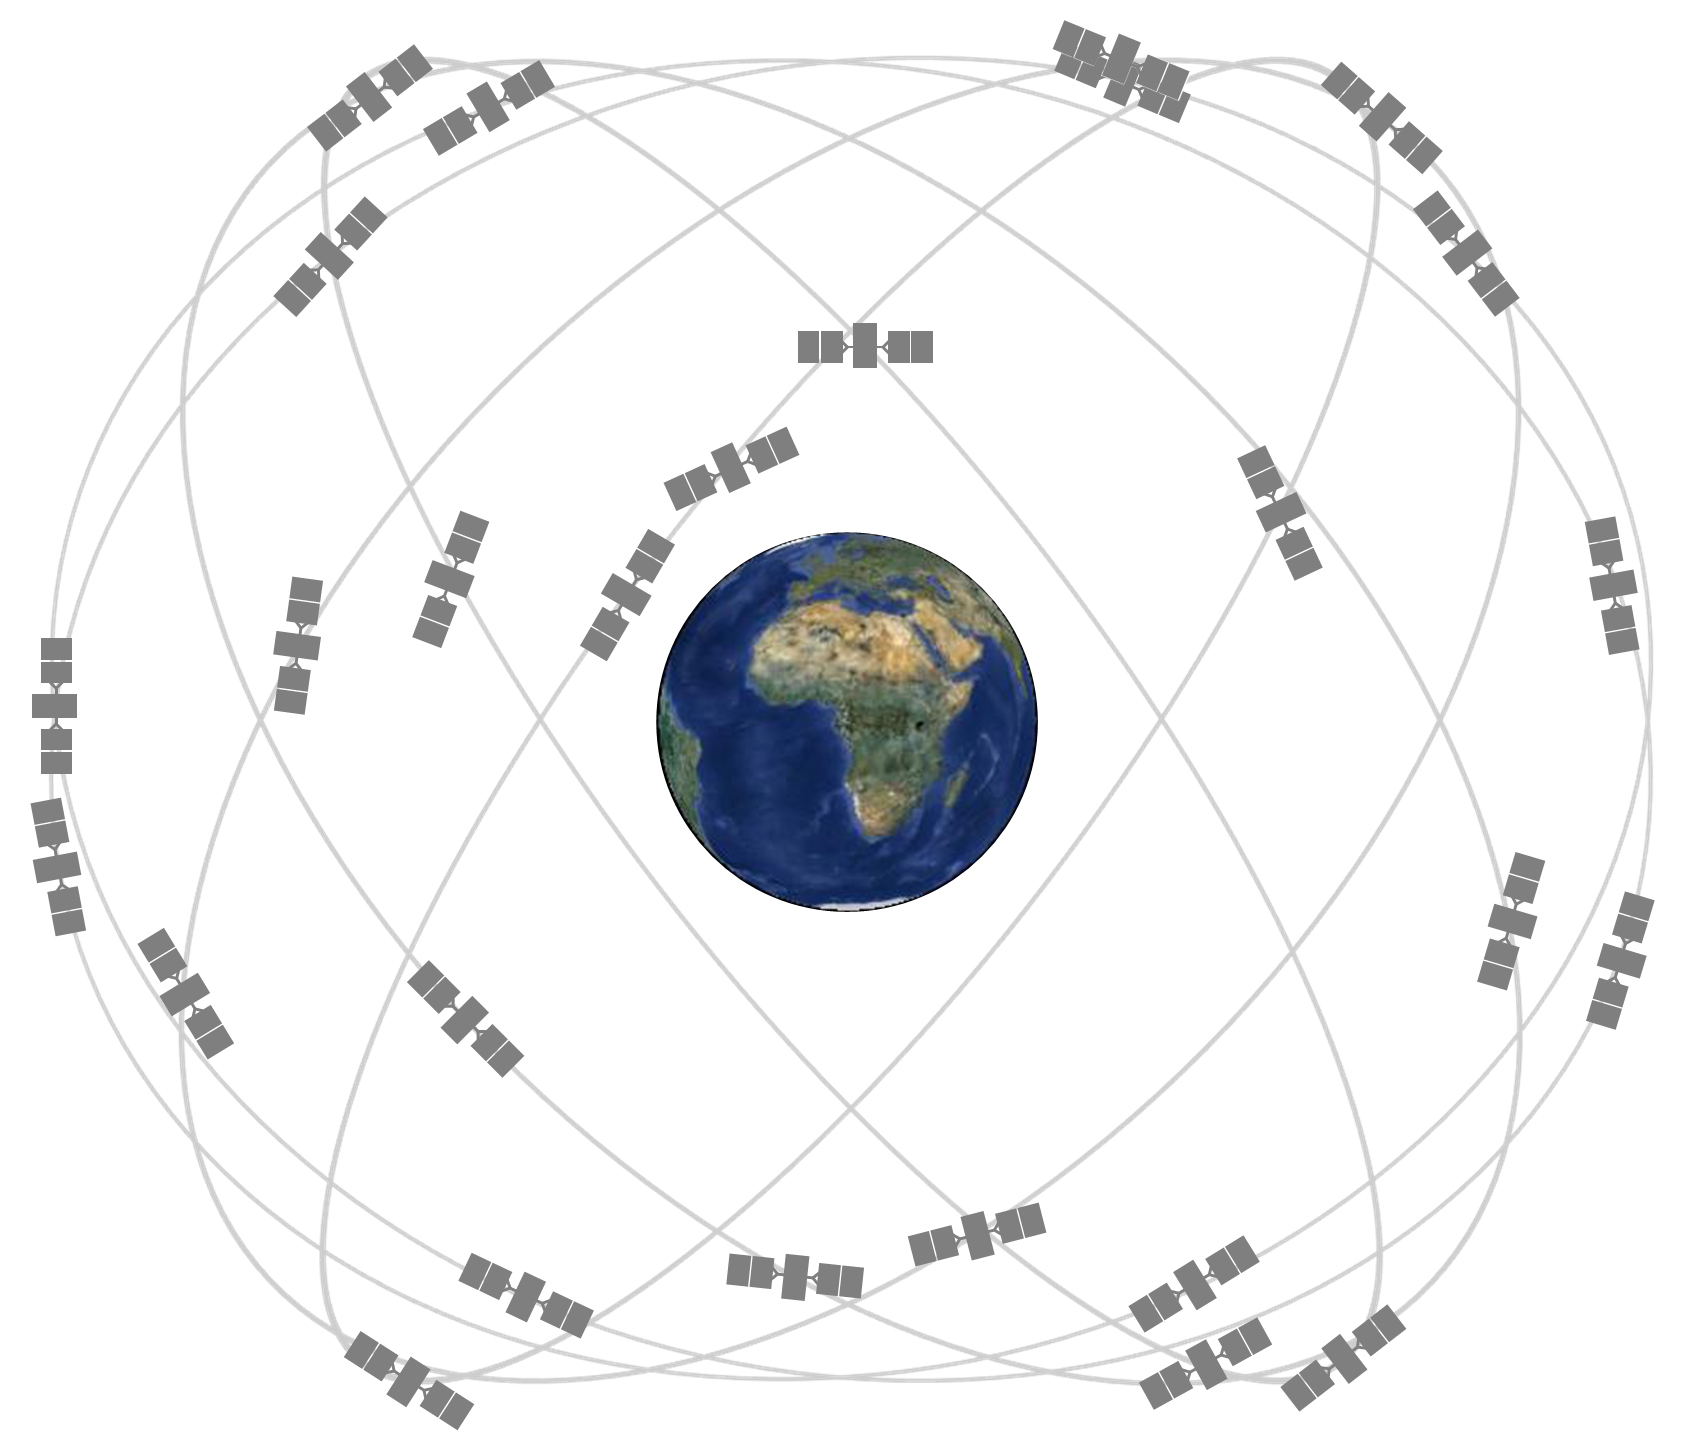
\includegraphics[width=100mm]{figs_chpt2/Fig3.jpg}	
	\caption[GPS satellite constellation.]{GPS satellite constellation (source: http://www.gps.gov/systems/gps/space/).}
	\label{fig:chpt2_fig3}
\end{figure}

\clearpage
\begin{figure}
	\centering
	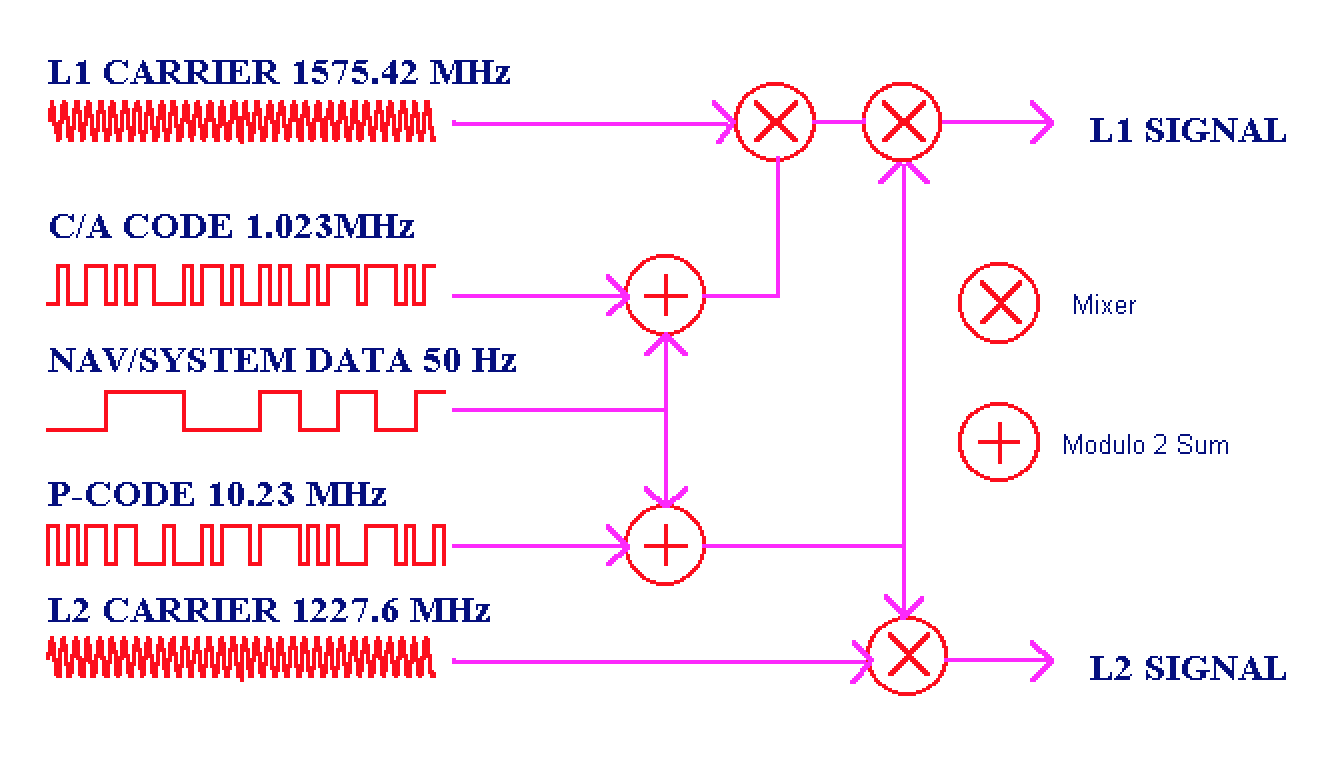
\includegraphics[width=100mm]{figs_chpt2/Fig4}	
	\caption[Composition of the signals from GPS satellites.]{Composition of the signals from GPS satellites (source: http://www.colorado.edu/geography/gcraft/notes/gps/gps.html).}
	\label{fig:chpt2_fig4}
\end{figure}

\clearpage
\begin{figure}
	\centering
	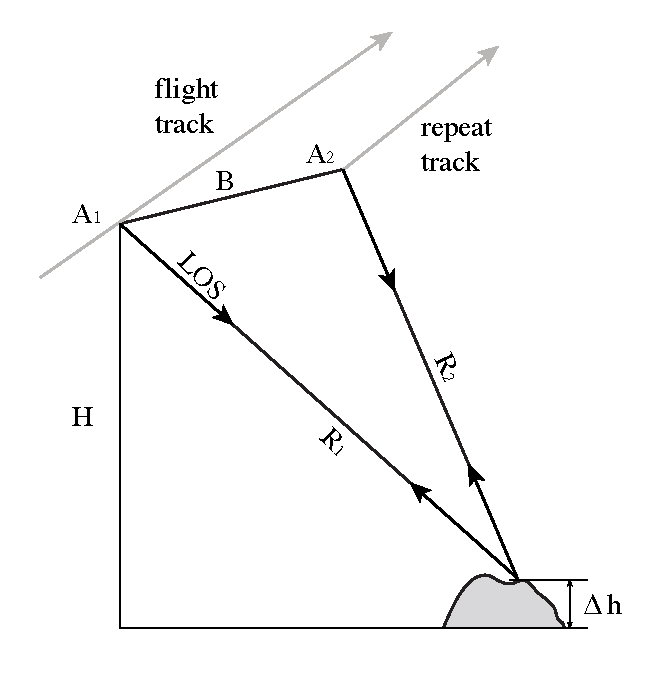
\includegraphics{figs_chpt2/Fig5}	
	\caption[Acquisition geometry of repeat-track interferometry.]{Acquisition geometry of repeat-track interferometry.  A1 and A2 are the antenna positions at the initial acquisition and second acquisition; R$_{1}$ and R$_{2}$  are the ranges from antenna A$_{1}$ and A$_{2}$ to the ground target; H is the flight height; B is the baseline; LOS is the line of sight of the radar beam; $\Delta h$ is the elevation of the ground target.}
	\label{fig:chpt2_fig5}
\end{figure}

\clearpage
\begin{figure}
	\centering
	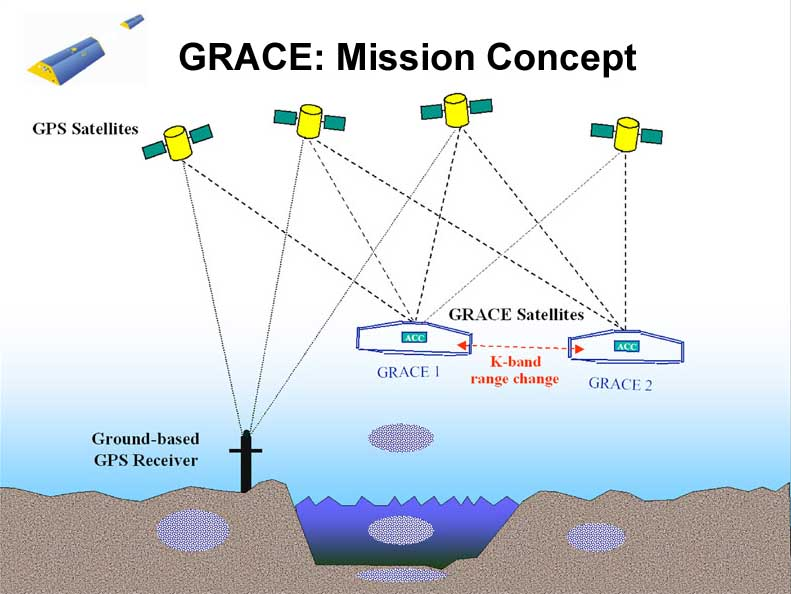
\includegraphics[width=100mm]{figs_chpt2/Fig6.jpg}	
	\caption[Basic mission concept of GRACE.]{Basic mission concept of GRACE (source: http://www.csr.utexas.edu/grace/publications/presentations/HPC2001.html).}
	\label{fig:chpt2_fig6}
\end{figure}

\clearpage
\begin{figure}
	\centering
	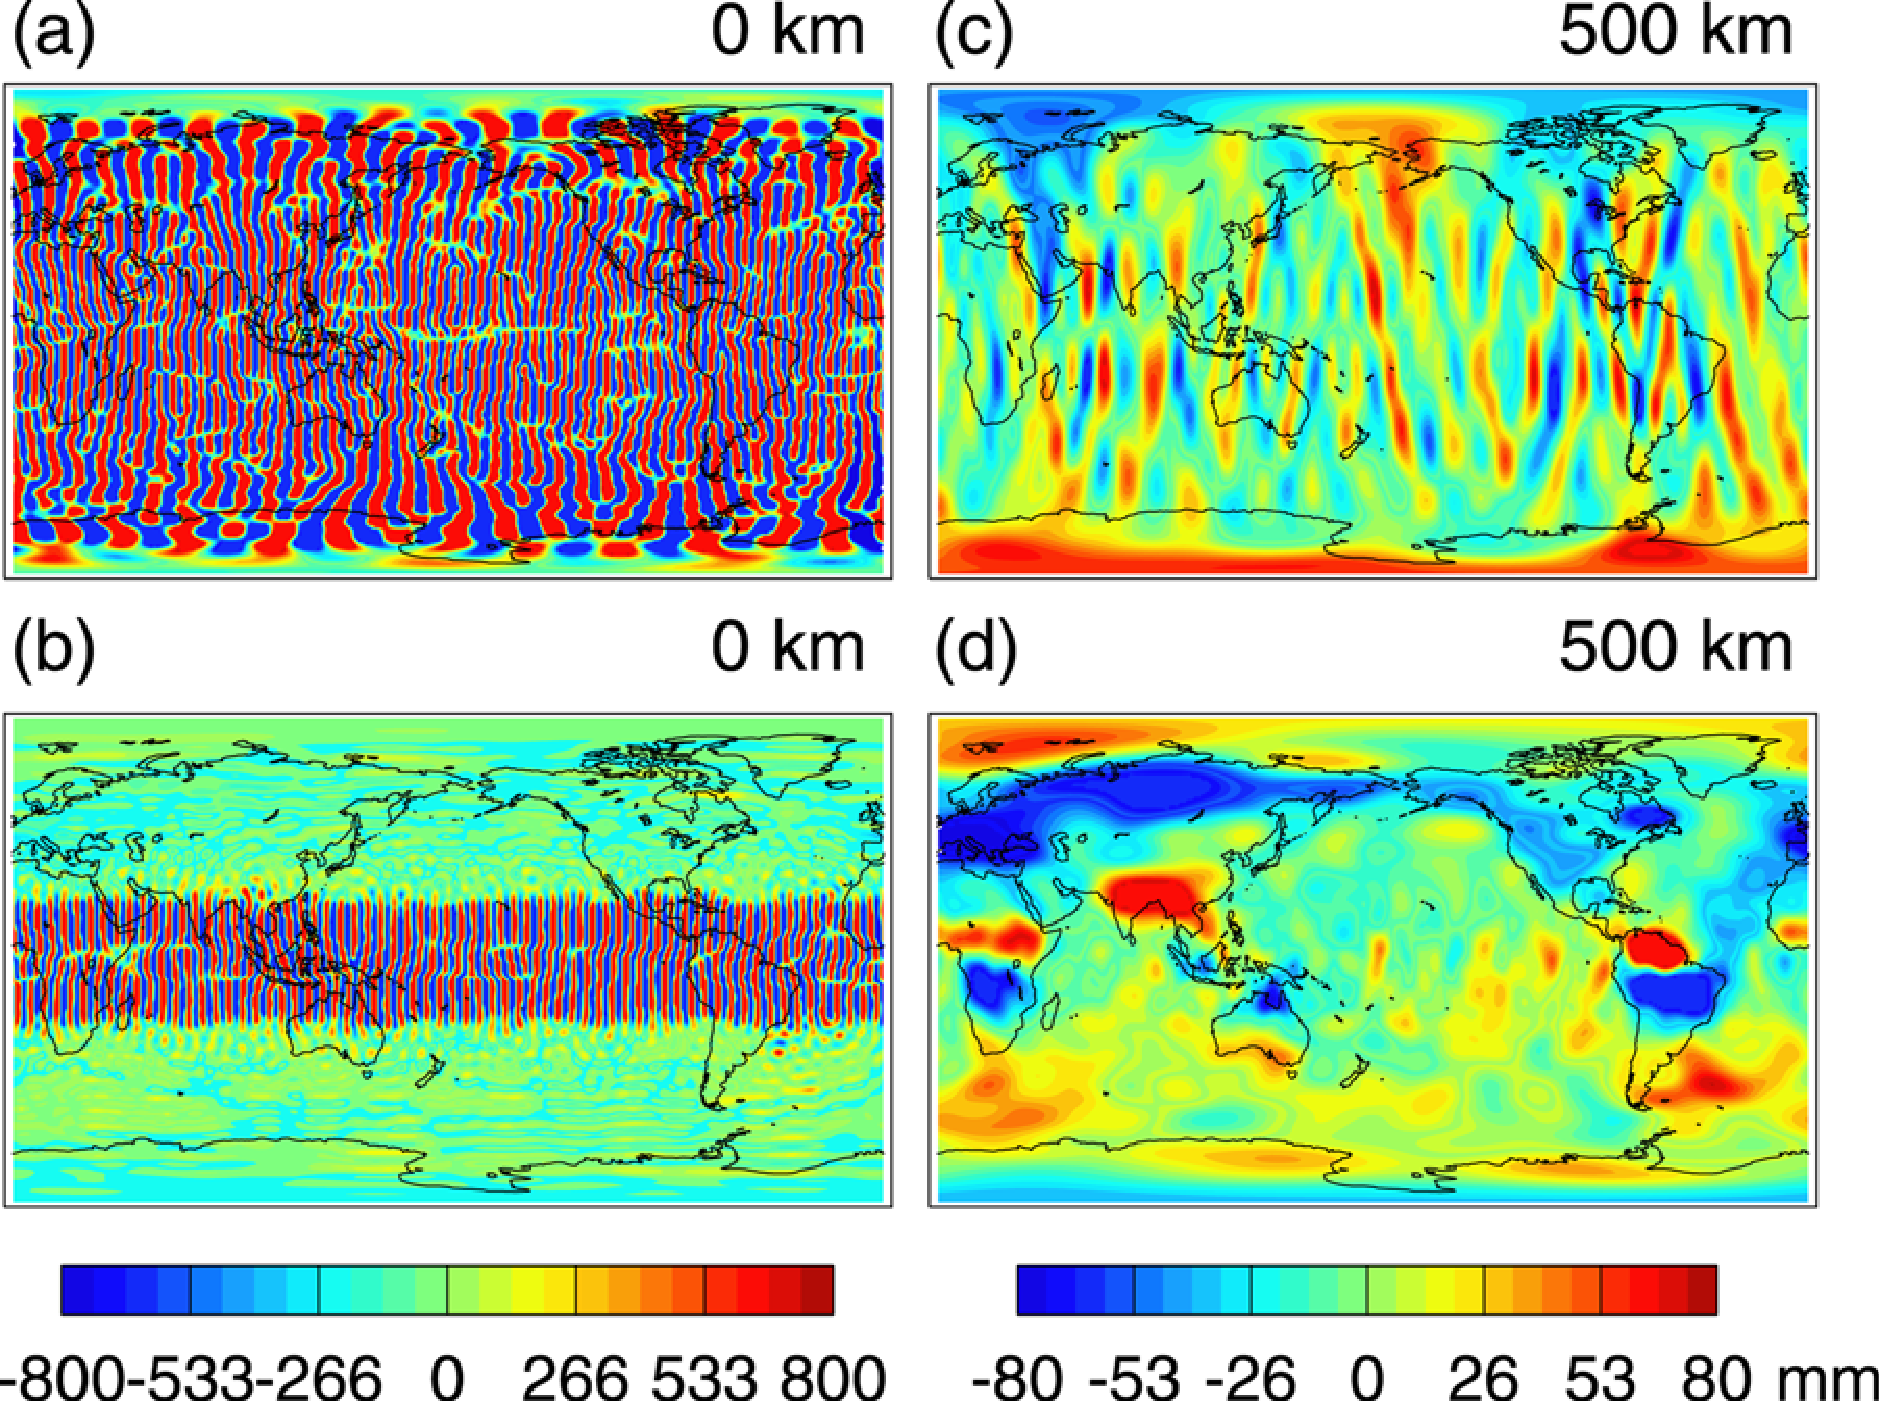
\includegraphics[width=100mm]{figs_chpt2/Fig7.pdf}	
	\caption[GRACE-derived maps of monthly anomaly of water storage.]{GRACE-derived maps of monthly anomaly of water storage. (a) Unsmoothed, no smoothing (b) filtered with correlated-error filter, no smoothing; (c) unfiltered and smoothed with 500 km Gaussian; (d) filtered with correlated-error filter and smoothed with 500 km Gaussian  (Figure 3 in \citet{swenson2006chpt2}). }
	\label{fig:chpt2_fig7}
\end{figure}